\subsection{Train/Dev/Test Sets}
We should always consider the fact that applied ML is an extremely iterative process with many parameters that affect our final outcome. It is virtually impossible to guess those parameters correctly in our first attempt. 
\begin{figure}[h]
    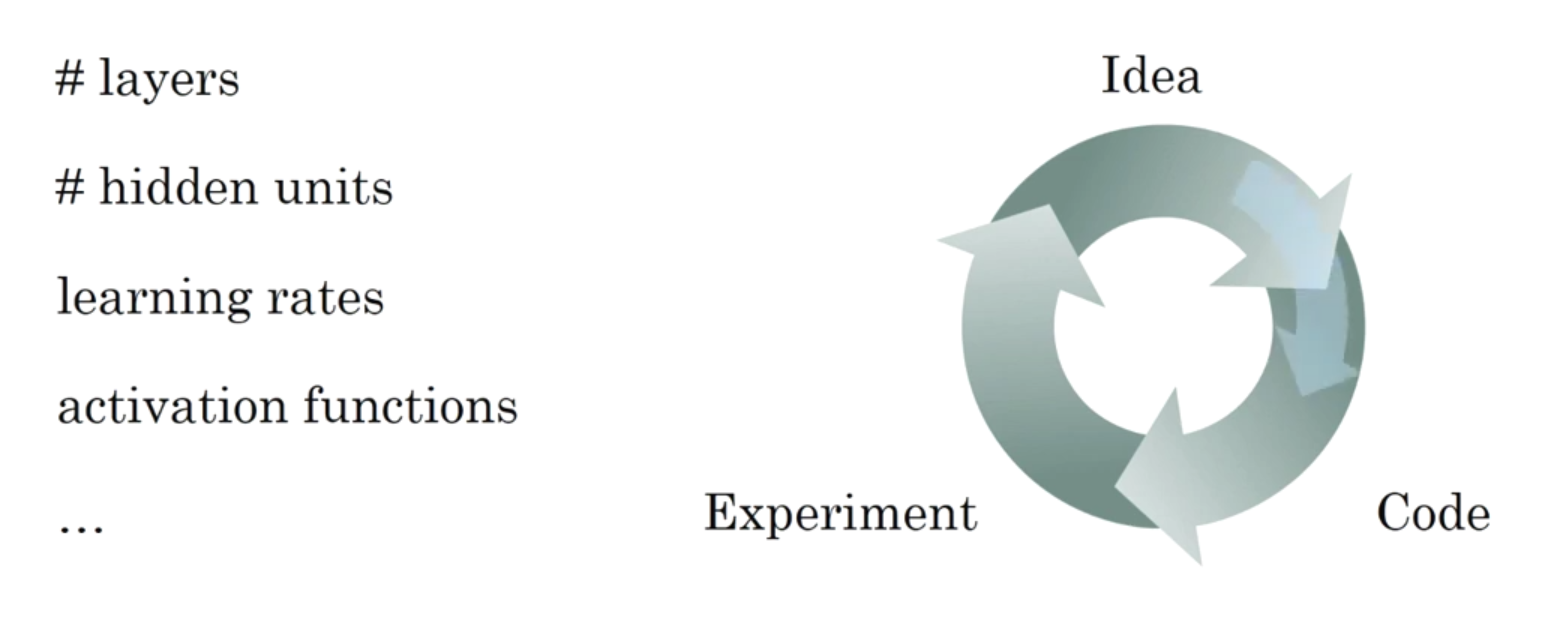
\includegraphics[scale=0.2]{images/iterative.png}
    \centering
\end{figure}

In the previous era of machine learning, it was common to divide all the data and split it according to a 70\%/30\% proportion, and assign them as your train and test sets respectively. Nowadays, however, with the emergence of big data, dev and test sets occcupy a smaller percentage of our data. For example, when we have a dataset with 100000 examples, an 20\% dev set is too big! As a result, the proportions nowadays look like 99.5\%/0.25\%/0.25\%. 

Not having a test set might be okay (only train/dev sets). 


\subsection{Bias/Variance}

The simplest explanation:
\begin{figure}[H]
    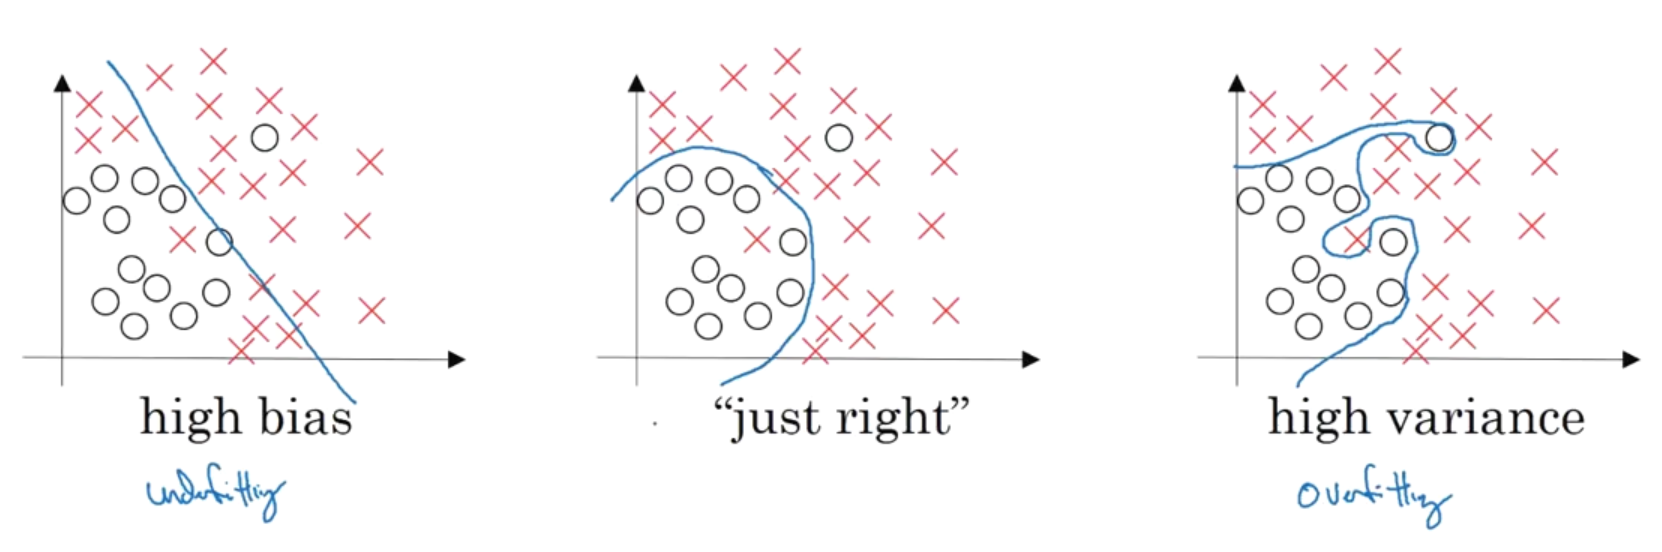
\includegraphics[scale=0.2]{images/biasvariance.png}
    \centering
\end{figure}

Consider another example for a cat classifer. 
\begin{table}[H]
    \begin{tabular}{|c|c|c|c|c|}
    \hline
                & High Variance & High Bias & \begin{tabular}[c]{@{}c@{}}High Bias\\ High Variance\end{tabular} & \begin{tabular}[c]{@{}c@{}}Low Bias\\ Low Variance\end{tabular} \\ \hline
    Train Error & 1\%           & 15\%      & 15\%                                                              & 0.5\%                                                           \\ \hline
    Test Error  & 11\%          & 16\%      & 30\%                                                              & 1.5\%                                                           \\ \hline
    \end{tabular}
\end{table}

The following classifier has both high bias and high variance. High bias because it is a mostly linear classifier, and it mostly underfits; high variance because in some occasions it shows overfitting behavior. 

\begin{figure}[H]
    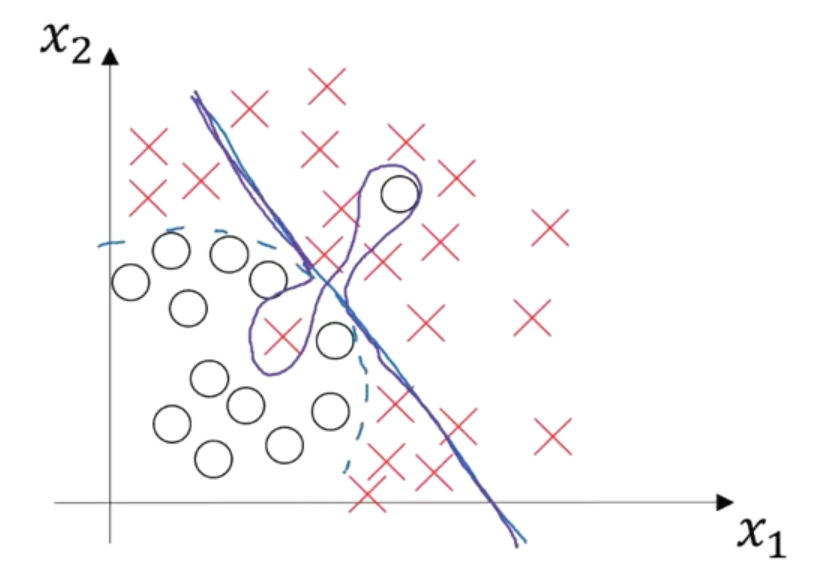
\includegraphics[scale=0.2]{images/highbv.png}
    \centering
\end{figure}

\subsection{Basic Recipe for Machine Learning}
\begin{figure}[H]
    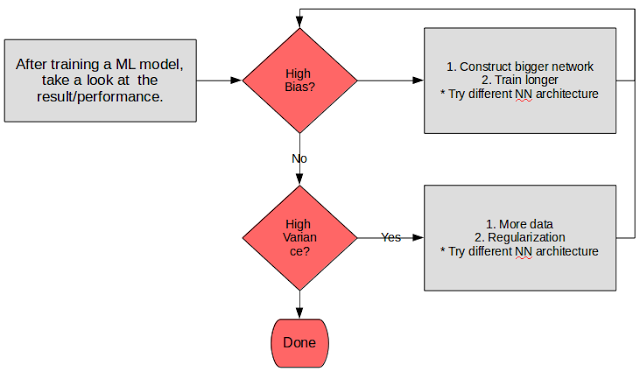
\includegraphics[scale=0.7]{images/recipe.png}
    \centering
\end{figure}

\subsection{Regularization}
If you suspect that your neural network has a high variance problem, meaning that it overfits your data, regularization is one of the first things you should try. The other option is to get more training data, but it is not always viable. 

Remember that in logistic regression, we were trying to minimize $J(w, b)$. Now we add the regularization term to the previous $J$.

$$
J(w, b) = \frac{1}{m}\sum_{i=1}^{m}{L(\yhat^{(i)}, y^{(i)})}+ \frac{\lambda}{2m} \norm{w}_2^{2}
$$ 

It's called $L_2$ regularization because it uses $L_2$ norm, which is: 

$$
\norm{w}_2^2 = \sum_{j=1}^{n_x} w_j^2 = w^T w
$$

It is also possible that we use $L_1$ regularization with the regularization term: 

$$
\frac{\lambda}{2m}\sum_{j=1}^{n_x} |w| = \frac{\lambda}{2m}\norm{w}_1
$$


Note that also a regularization term for bias is possible, but since $b$ is not as high-dimentional as $w$, its regularization term, which is equal to $\frac{\lambda}{m}b^2$, is usually omitted.

In a more complex neural network, though, a more generalized equation will be like this: 

$$
J(W\lay{1}, b\lay{1}, \dots, W\lay{L}, b\lay{L}) = \frac{1}{m}\sum_{i=1}^{m}{L(\yhat^{(i)}, y^{(i)})} + \frac{\lambda}{2m} \sum_{l=1}^L \norm{W\lay{l}}_F^2
$$

$\norm{W\lay{l}}_F^2$ is called the \emph{Frobenius Norm} of the matrix $W\lay{l}$, and knowing that the shape of $W\lay{l}$ is $(n\lay{l-1}, n\lay{l})$ it's computed like this: 

$$
\norm{W\lay{l}}_F^2 = \sum_{i=1}^{n\lay{l-1}} \sum_{j=1}^{n\lay{l}} \Big(w_{ij}^{[l]}\Big)^2
$$

Regularization is also applied to the gradients (it is called \emph{weight decay}): 
$$
dw\lay{l} = (from\ backprop) + \frac{\lambda}{m}w\lay{l}
$$

\subsection{Why Regularization Reduces Overfitting}
Consider a situation where you have a neural network that overfits your data. Remember the original non-regularized cost function: 

$$
J = \frac{1}{m}\sum_{i=1}^{m} L(\yhat^{(i)}, y^{(i)})
$$

In order to reduce overfitting, we penalized $J$ with a regularization term: 
$$
J = \frac{1}{m}\sum_{i=1}^{m} L(\yhat^{(i)}, y^{(i)}) + \frac{\lambda}{2m}\sum_{l=1}^L \norm{W\lay{l}}_F^2
$$

\textbf{Intuition:} If we set $\lambda$ to be a really big number, our minimization algorithm will seek to set $W\lay{l} = 0$, which essentially means that a lot of hidden units will be zeroed out, which means that their impact will be reduced, and we will end up with a simpler neural network that is closer to the "High Bias" realm than it is to the "High Variance" realm.

\textbf{Another Intuition:} Consider using hyperbolic tangent as the activation function. If we regularize our weights, they will become smaller, and as a result, $z = wx+b$ will be smaller. With smaller $z$s, we will be wandering in the "linear section" of $tanh$, which means that each layer will be \emph{roughly} linear, which leaves our network having higher bias. 

\begin{figure}[H]
    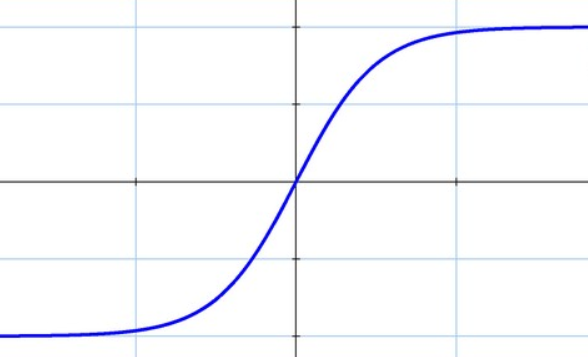
\includegraphics[scale=0.2]{images/tanh.png}
    \centering
\end{figure}